\documentclass[../reportesINE.tex]{subfiles}

\begin{document}

\subsection{Inicio del desarrollo}
Cuando me asignaron este desarrollo, la orden fue: "Hacer un módulo de consulta y reportes para cada sitema, el usuario debe ser capaz de filtrar los datos como a él mejor le convenga". Los primeros problemas con los que me enfrente fueron: 
\begin{itemize}
\item La cantidad de datos, que se iban a acumular con el tiempo, si llamabamos con una sola petición a la carga de todos los datos el módulo tardaría mucho en cargar. 
\item ¿Qué datos iba a poder consultar el usuario? Pues en la base hay datos que sólo son de interés para la aplicación, por ejemplo: bandera activo para los estatus de los registros, al usuario sólo le interesa saber el estatus actual.
\item ¿Cómo iban a ser las consultas a la base? ¿Se construirían al vuelvo, según los datos solicitados? ¿Se tendría una consulta estática y sólo se agregarían filtros y se seleccionarían las columnas necesarías?
\end{itemize}
Lo anterior se resumía en un sólo problema: ¿Cómo iba a manejar los datos?, construir consultas al vuelo además de ser un reto un tanto complicado no era óptimo en el siguiente escenario: \\ \\
\textit{Generas un reporte con n número columnas y con m número de condiciones (filtros), vuelves a generar el reporte con n+1 número de columnas y m número de condiciones. Internamente lo que haría el sistema es generar una consulta para la primera petición y entregar el resultado, con la segunda petición repetir el proceso.} \\ ¿Por qué generar dos veces una consulta prácticamente idéntica? \\ \\
El analista de mi equipo me hizo llegar una lista especifíca de campos a consultar por cada sistema, esto simplificó el trabajo pues al saber que se quería consultar cree vista a nivel de base de datos para cada sitema con los datos requeridos. Teniendo todo concentrado en una vista las consultas se harían a una sola tabla y no tendría que preocuparme por las uniones,  sin embargo seguía con el problema de la construcción de la consulta. \\ \\
En cuanto al manejo de la cantidad de datos, decidí implementar páginación. La peticiones regresarían de n en n los datos, según el número de petición. 


\subsection{Versión 1.0}
Esta versión fue el desarrollo más básico del requerimiento solicitado, el alcance consistió en mostrar datos según el sistema seleccionado. 

\subsubsection{La capa de persistencia}
Al concentrar todos los datos en vistas por sistema, se crearon las clases (mapeos de las vistas en base de datos con el Hibernate): 
\begin{itemize}
\item ReporteDISCIPLINARIOS
\item ReporteSIDJ
\item ReporteSIMI
\item ReporteSISEROG
\end{itemize}

\subsubsection{El DAO}
Para cada clase de la persisntencia se crearon sus respectivos DAO:  
\begin{itemize}
\item DAOReporteDISCIPLINARIOS
\item DAOReporteSIDJ
\item DAOReporteSIMI
\item DAOReporteSISEROG
\end{itemize}

\subsubsection{La capa de negocio}
Para esta versión como se trataba de módulos independientes se crearon clases de negocio para cada DAO:
\begin{itemize}
\item BSDReporteDISCIPLINARIOS
\item BSDReporteSIDJ
\item BSDReporteSIMI
\item BSDReporteSISEROG
\item ASReporteDISCIPLINARIOS
\item ASReporteSIDJ
\item ASReporteSIMI
\item ASReporteSISEROG
\end{itemize}

Las capas del DAO y negocio con los métodos de consulta necesarios para el paginado:
obtenerListaDeDatos(filtros, indice inicial, indice final, tamaño de página): Obtiene n datos de una vista entre los índices inicial y final con ciertos filtros. Donde n es el tamaño de página. Si no se cuenta con filtros regresa todos los datos de la vista.
obtenerTotalDeRegistros(filtros): Obtiene el número total de registros de una vista con ciertos filtros. Si no cuenta con filtros regresa el total de datos de la vista. 

\subsubsection{La capa de control}
Se crearon controladores para cada vista de la aplicación: 
\begin{itemize}
\item MBReporteDISCIPLINARIOS
\item MBReporteSIDJ
\item MBReporteSIMI
\item MBReporteSISEROG
\end{itemize}

\subsubsection{La capa de presentación}
Al WAR de Consulta del  \textit{Sistema Integral de la Dirección Jurídica} se le agregaron las vistas: 
\begin{itemize}
\item menuReportes
\item reportesDISCIPLINARIOS
\item rerpotesSIMI 
\item reportesSIDJ
\item reportesSISEROG
\end{itemize}
Mostrando los datos con el componente:
DataTable - Paginator de PrimeFaces\footnote{http://www.primefaces.org/showcase/ui/data/datatable/paginator.xhtml}.

\subsection{Entrega versión 1.0}
La primera versión del módulo constaba de un ménu donde se seleccionaba el sistema a consultar \textit{Imagen \ref{fig:menuUno}}, al seleccionar la opción deseada el usuario era redirigido a una pantalla con una tabla de datos correspondientes al sistema seleccionado \textit{Imagen \ref{fig:versionUno}}. 

\begin{figure}[h]
  \centering
  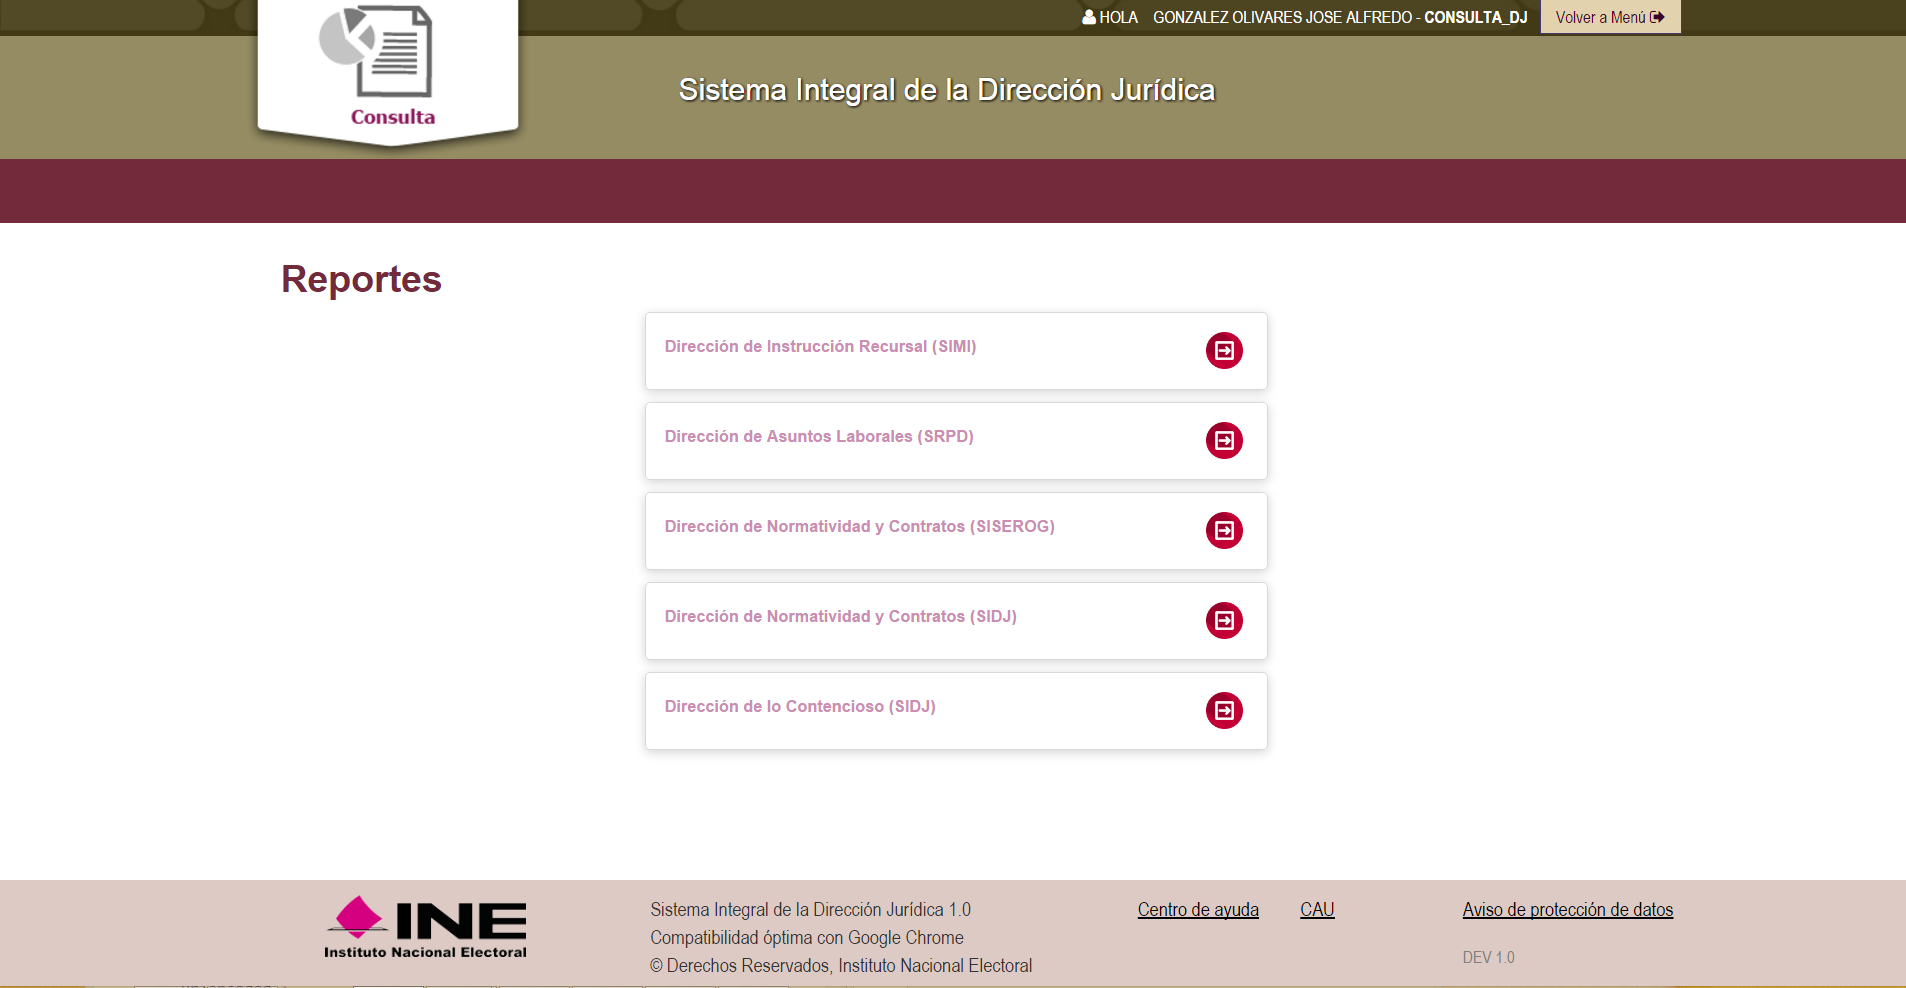
\includegraphics[width=\linewidth]{img/menuUno.png}
  \caption{Menú selección de sistemas para consulta y reportes. }
  \label{fig:menuUno}
\end{figure}

\begin{figure}
  \centering
  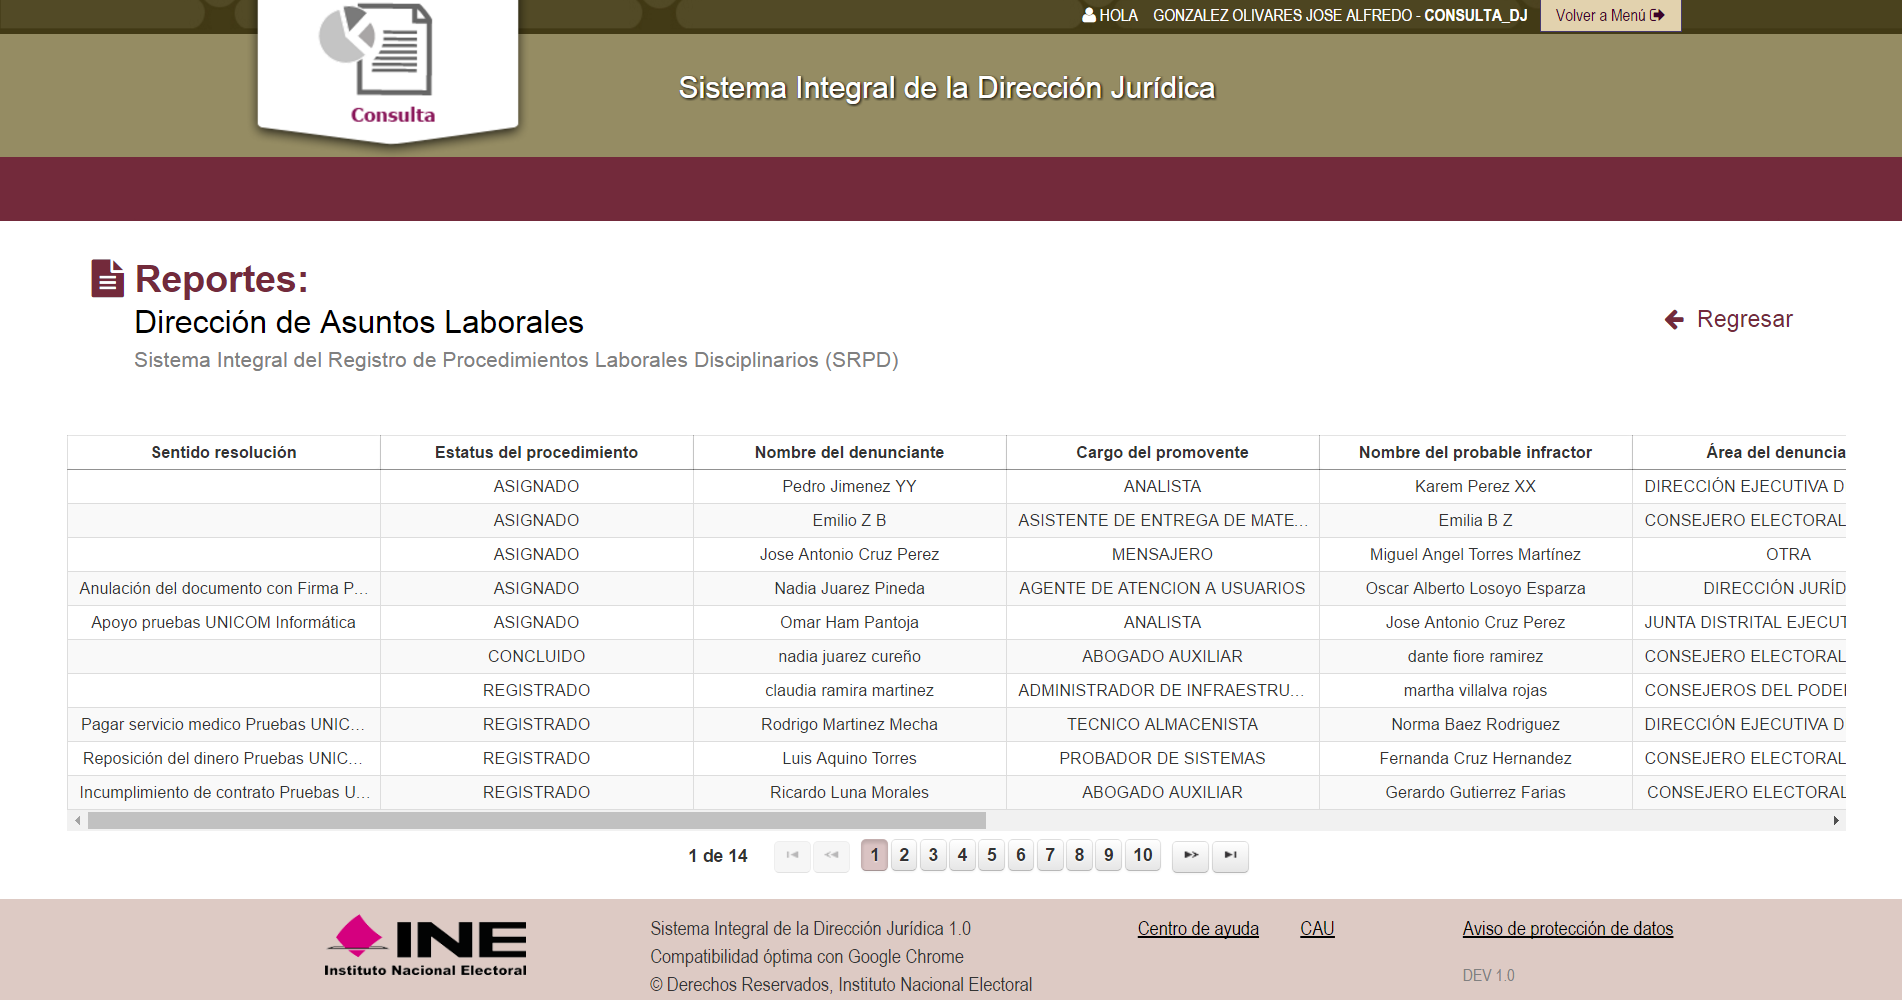
\includegraphics[width=\linewidth]{img/versionUno.png}
  \caption{Ejemplo panalla de consulta versión 1.0. }
  \label{fig:versionUno}
\end{figure}

\subsection{Versión 1.1}
Para esta versión era necesario agregar filtros a cada columna y la exportación de datos a excel. El desarrollo sólo presento cambios en \textit{La capa de presentación}. 

\subsubsection{La capa de presentación}
En cada vista se agrega el componente, para exportación de datos:  
DataExporter - Basic de PrimeFaces\footnote{http://www.primefaces.org/showcase/ui/data/dataexporter/basic.xhtml}. 
Y para el filtrado de columnas: 
DataTable - Filter de PrimeFaces\footnote{http://www.primefaces.org/showcase/ui/data/datatable/filter.xhtml}.

\subsection{Entrega versión 1.1}
El menú de selección de sistema no fue modificado y ahora cada columna en la tabla de datos tenía en el encabezado un campo para capturar texto, este texto servía como filtro para la columna correspondiente. Además se agregó la opción de descarga en cada tabla \textit{Imagen \ref{fig:tablaV2}}.

\begin{figure}[h]
  \centering
  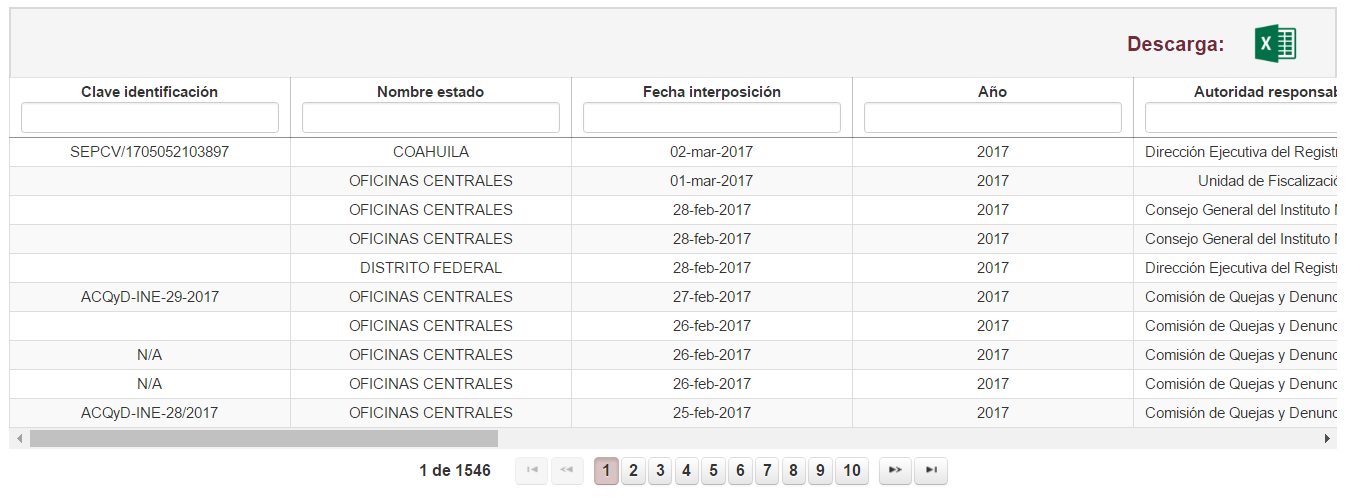
\includegraphics[width=\linewidth]{img/tablaV2.PNG}
  \caption{Ejemplo de tabla de datos para el módulo de consulta versión 1.1.}
  \label{fig:tablaV2}
\end{figure}

\subsection{Versión 2.0}
Con la \textit{versión 1.1} ya se cubrían todos los requerimientos para su entrega final, sin embargo el desarrollo contaba con "detalles" importantes que no se podían dejar a un lado: 
\begin{itemize}
\item El filtrado de datos era demasiado ineficiente, pues el componente cada que se presionaba una tecla mandaba una petición al servidor para filtrar, es decir: Si querías filtrar sobre una columna la palabra abogado, el módulo buscaba los datos correspondientes con letra a, luego con letra b, o, .... y así sucesivamente. \\ Para el usuario final era muy incómodo pues tenía que esperar a que la búsqueda sobre todos los datos existentes se efectuará letra por letra. 
\item Los filtros estaba muy limitados, sólo se podía buscar por coincidencia de texto, el buscar por rango de fechas no era posible, de igual manera si se deseaba limitar la búsqueda por palabra exacta para alguna columna. 
\item En caso de querer agregar más filtros o columnas de datos en el módulo a algún sistema, era muy tardado y complicado pues afectaba a cada una de las capas del desarrollo. En pocas palabras dar mantenimiento resultaba tedioso y complicado. 
\end{itemize}
El módulo de reportes estaba desarrollado de tal forma que cada sistema contaba con su propia implementación, pero ¿Por qué un desarrollo para cada sistema y no uno genérico? esta fue la motivación para el desarrollo de la \textit{versión 2.0}   \\ \\
En esta implementación se arregló lo antes mencionado, fue necesario rehacer todo el desarrollo excepto la \textit{capa de persistencia}. 

\subsubsection{El DAO y la capa de negocio}
Para estas capas todas las clases de la \textit{versión 1.0} fueron sustituidas por una clase: \textit{DAOReportes}, con dos métodos: 

\begin{itemize}
\item obtenerListaDeDatos(filtros, indice inicial, indice final, tamaño de página, identificador de reporte)
\item obtenerTotalDeRegistros(filtros, identificador de reporte)
\end{itemize}

Sólo se agrego el parámetro \textit{identificador de reporte}, a los métodos que se tenían en las clases de la \textit{versión 1.0}. 

\subsubsection{La capa de control y la capa de presentación}
Las clases de la \textit{versión 1.0} fueron sustituidas por: \textit{MBReportes}, para la capa de control y un sólo archivo \textit{reportes.xhtml} para la capa de presentación. 
Para poder tener una sola capa de presentación se creo la clase \textit{Column}, con los siguientes atributos: 
\begin{itemize}
\item Título, nombre con el que el usuario identifica la columna.  
\item Contenido, nombre con el que la columna esta identificada a una vista en base de datos.
\item Filtro , tipo de filtro de la columna (entero, cadena, opción)
\item Opciones, si se deseaba filtrar sólo por opciones en especifico aquí son listadas.
\end{itemize}
Está clase sólo cuenta con métodos de tipo constructor, se pudiera ver esta clase como una envoltura para generalizar columnas.  \\ \\
Así para cada vista  para los reportes, una por sistema,  que se tiene en la base de datos, se crea una lista de columnas. Por ejemplo: \textit{Imagen \ref{fig:ejemploColumna}}. \\ \\
El problema de mantenimiento del módulo y el exceso de código repetido que tenían las versiones anteriores fue solucionado, con esta nueva implementación se tiene menos líneas de código y además agregar y eliminar columnas para los 
reportes es muy sencillo, se agregan o eliminan datos de la lista correspondiente. \\ \\
La capa de presentación es generada de forma dinámica según la lista de columnas a las que se desee acceder. 

\begin{figure}[h]
  \centering
  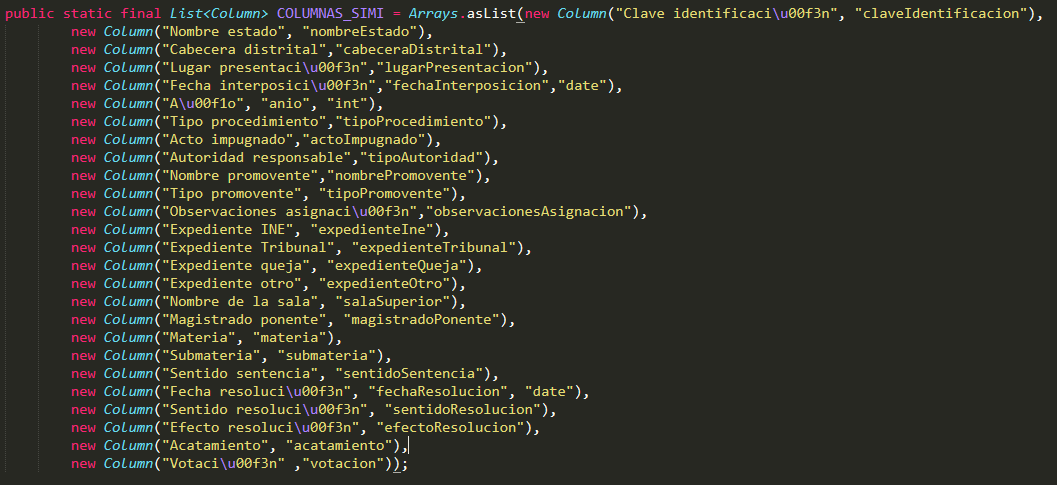
\includegraphics[width=\linewidth]{img/ejemploColumna.PNG}
  \caption{Ejemplo de lista de columnas disponibles para reportes del Sistema Integral de Medios de Impugnación. }
  \label{fig:ejemploColumna}
\end{figure}


\subsection{Entrega versión 2.0}
El menú de \textit{versión 1.0} no fue modificado. Ahora ya no se muestra una tabla con todos los datos disponibles en la vista, primero se pide al usuario seleccionar las columnas que le son de importancia y si desea aplicar un filtro sobre la opción seleccionada después se presiona el botón de aplicar. Una vista previa se despliega con los datos solicitados y la opción de exportar a excel  \textit{Imagen \ref{fig:ejemploModuloCompleto}}.  

\begin{figure}[h]
  \centering
  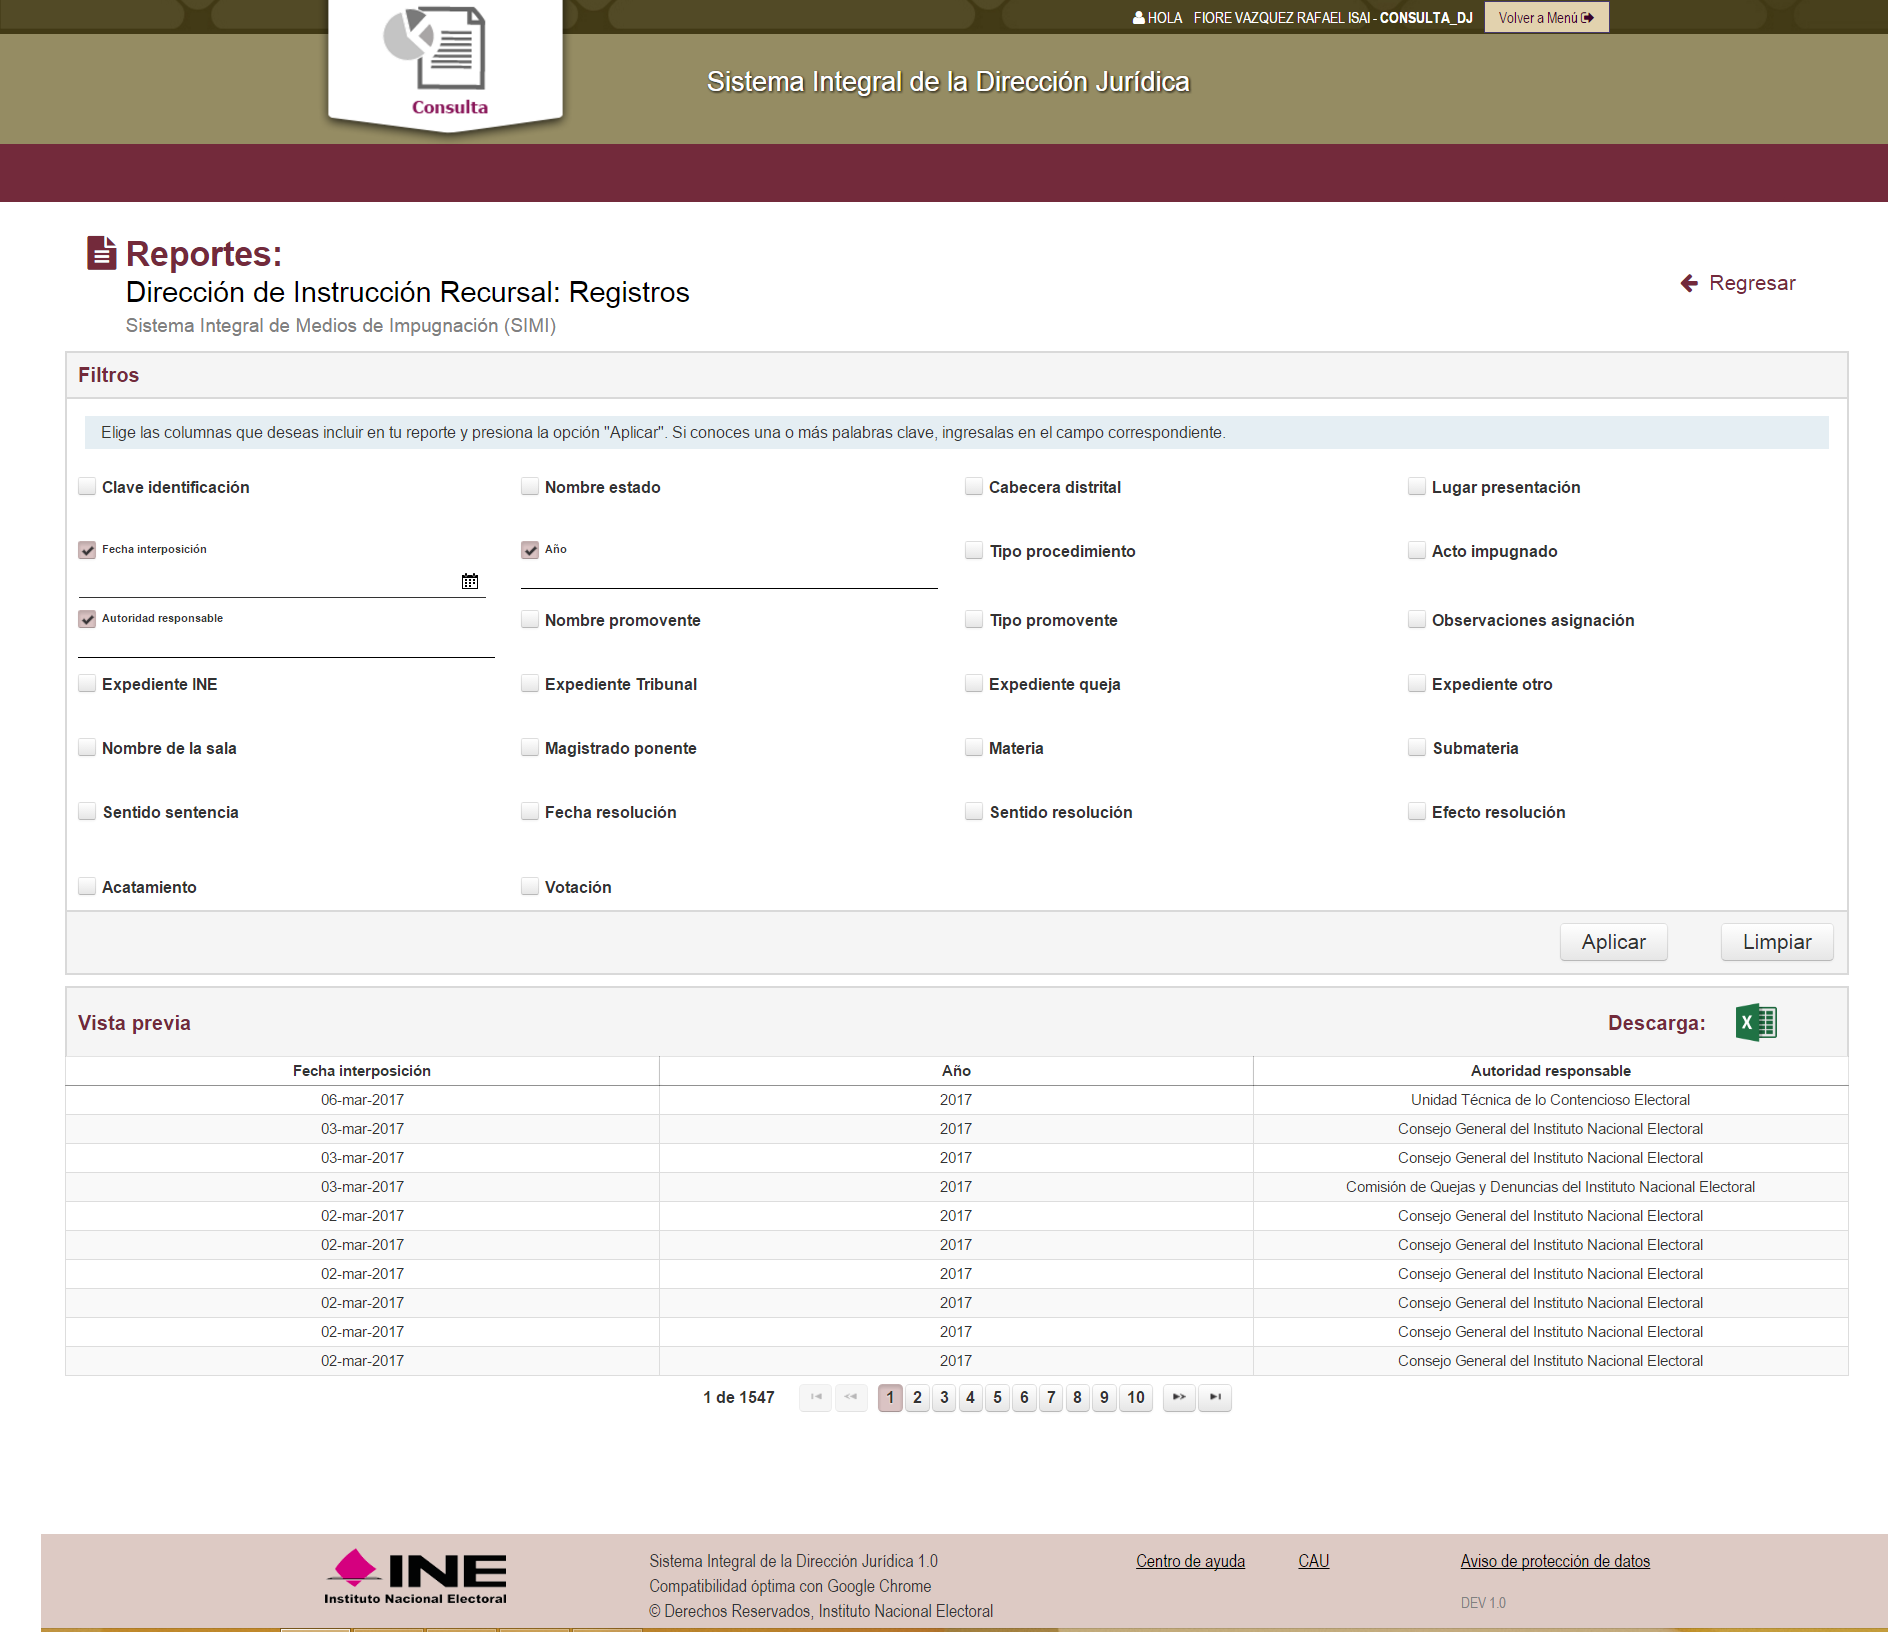
\includegraphics[width=\linewidth]{img/ejemploModuloCompleto.png}
  \caption{Ejemplo panalla de consulta versión 2.0. }
  \label{fig:ejemploModuloCompleto}
\end{figure}





\end{document}